\DiaryEntry{Interesting Integrals, Part 8}{2019-08-01}{Integrals}

We want to solve

\bee
I = \int x^3 \sqrt{1-x^2} dx
\eee

and start with a substitution approach

\bee
u = 1-x^2 \rightarrow du=  -2x dx \rightarrow dx = -\frac{du}{2x}, x^2 = 1-u, x^3 = (1-u) \sqrt{1-u}
\eee

which yields

\begin{align*}
I &= \int x x^2 \sqrt{1-x^2} dx = - \frac{1}{2} \int x (1-u) \sqrt{u} \frac{du}{x} = - \frac{1}{2} \int (1-u) \sqrt{u} du \\ &= - \frac{1}{2} \int u^{1/2} - u^{3/2} du = \frac{u^{5/2}}{5} - \frac{u^{3/2}}{3} = \frac{(1-x^2)^{5/2}}{5} - \frac{(1-x^2)^{3/2}}{3}
\end{align*}

\qed

A plot of the integrand can be found below.

\begin{figure}[hbt!]
\centering
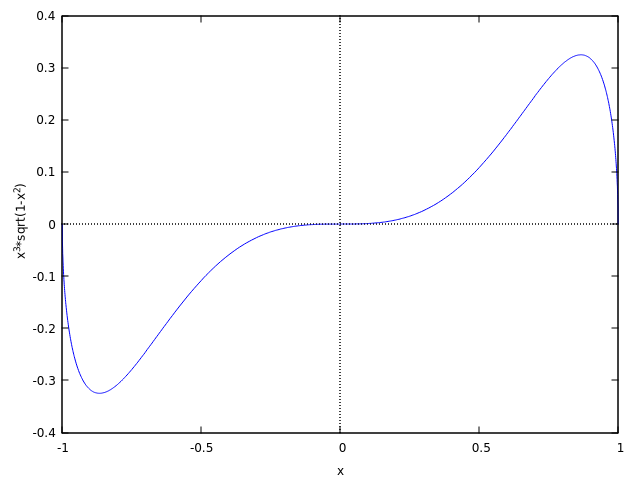
\includegraphics[scale=0.5]{images/interesting_integrals_08_1.png}
\end{figure}




Maybe a bit more interesting is the slightly different integral

\bee
I = \int x^2 \sqrt{1-x^2} dx
\eee

Here we make a trigonometric substitution,

\bee
x = \sin u \rightarrow \frac{dx}{du} = \cos u \rightarrow dx = \cos u du, u = \arcsin x
\eee

which yields

\bee
I = \int \sin^2 u \sqrt{1-\sin^2 u} \cos u du = \int \sin^2 u \cos^2 u du = \frac{1}{4} \int \sin^2 2u du
\eee

where we used some trigonometric magic in the last step.

This last integral can (surprinsingly) be solved in closed-form by means of partial integration. We have $\int u' v = uv - \int u v'$ with

\bee
u' = \sin x \rightarrow u = - \cos x, v = \sin x \rightarrow v' = \cos x
\eee

and obtain

\begin{align*}
\int \sin^2 u du &= - \cos u \sin u - \int (- \cos u) \cos u du = - \cos u \sin u + \int \cos^2 u du \\ &= - \cos u \sin u + \int 1 - \sin^2 u du = - \cos u \sin u + u - \int \sin^2 u du
\end{align*}

This we can "solve" for the desired integral,

\bee
\int \sin^2 u du = \frac{1}{2} \left( u - \sin u \cos u \right) \qed
\eee

and now we can continue with the original integral,

\begin{align*}
I &= \frac{1}{4} \int \sin^2 2u du = \frac{1}{4} \int \sin^2 v \frac{dv}{2} = \frac{1}{8} \int \sin^2 v dv = \frac{1}{16} \left[ v - \sin v \cos v \right] \\ &= \frac{1}{16} \left[ 2u - \sin 2u \cos 2u \right] = \frac{u}{8} - \frac{\sin 2u \cos 2u}{16}
\end{align*}

We need some more trigonometric magic to get rid of the $2u$ terms,

\bee
I = \frac{u}{8} - \frac{\sin u \cos u (1 - 2\sin^2 u)}{8} = \frac{\arcsin x}{8} - \frac{x \sqrt{1-x^2} (1-2x^2)}{8} \qed
\eee

A Figure of the integrand can be foud below.

\begin{figure}[hbt!]
\centering
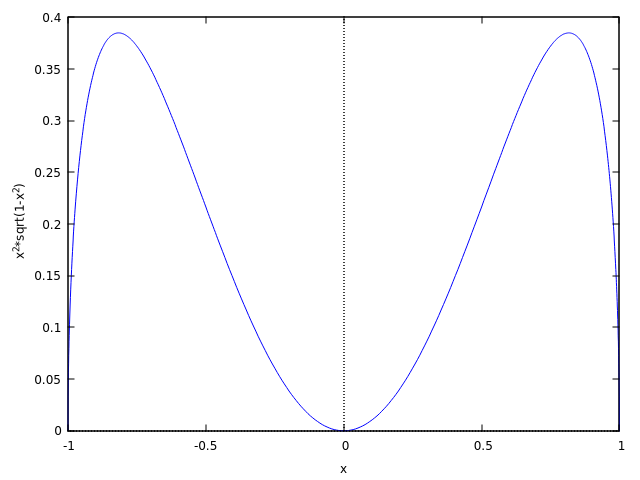
\includegraphics[scale=0.5]{images/interesting_integrals_08_2.png}
\end{figure}



%%% Local Variables:
%%% mode: latex
%%% TeX-master: "journal"
%%% End:
